\documentclass[a4paper,14pt,russian]{report}
\usepackage[utf8]{inputenc}
\usepackage[T2A]{fontenc}
\usepackage{extsizes}
\usepackage{amsmath}
\usepackage{listings}
\usepackage{xcolor}
\usepackage{tabularx}
\usepackage{geometry}
\usepackage{titlesec}
\usepackage{graphicx}
\usepackage[font=small,labelfont=bf]{caption}
\usepackage{indentfirst}

\newcommand{\insertInstitute}{
  Институт компьютерных наук и технологий\linebreak
  Кафедра «Информационные системы и технологии»
}
\newcommand{\insertTitle}{ОТЧЕТ\par по дисциплине «Инженерная и компьютерная графика»\par \textbf{Построение и оцифровка 2D графиков}}
\newcommand{\insertAuthor}{С А. Новиков}
\newcommand{\insertAuthorPosition}{студент гр 13532/1}
\newcommand{\insertVerifier}{А А. Ефремов}
\newcommand{\insertVerifierPosition}{доцент, кф.-м.н}

\newcommand{\sectionbreak}{\clearpage}
\newcommand{\subsectionbreak}{\clearpage}

\graphicspath{ {./images/} }
\renewcommand{\figurename}{Рисунок}
\renewcommand{\tablename}{Таблица}

\sloppy

\linespread{1.3}
\definecolor{lightgray}{gray}{0.95}
\renewcommand{\contentsname}{Содержание}
\renewcommand{\thesection}{\arabic{section}}
\newgeometry{left=3cm,right=2cm,top=2cm,bottom=2cm}
\setlength{\parindent}{1.25cm}
\lstset{
  backgroundcolor=\color{lightgray},
}


\begin{document}

\pagenumbering{gobble}
\begin{center}
  Министерство науки и высшего образования РФ\linebreak
  Санкт-Петербургский политехнический университет\linebreak
  Петра Великого\linebreak
  \insertInstitute\linebreak
\end{center}
\vspace{1.5cm}
\begin{tabularx}{\textwidth}{Xr}
  УДК $\rule{4cm}{0.15mm}$ & УТВЕРЖДАЮ \\
                           & $\rule{5cm}{0.15mm}$ \\
                           & $\rule{5cm}{0.15mm}$ \\
                           & $\rule{5cm}{0.15mm}$ \\
                           & «$\rule{0.8cm}{0.15mm}$» $\rule{2cm}{0.15mm}$ $\rule{1.1cm}{0.15mm}$ г. \\
\end{tabularx}
\vspace{1.5cm}
\begin{center}
  \insertTitle\par
\end{center}
\vspace{1.5cm}
\begin{tabularx}{1\textwidth}{Xll}
  \textbf{Выполнил:}    & & \\
  \insertAuthorPosition & $\rule{3.5cm}{0.15mm}$ & \insertAuthor \\
                        & подпись, дата & \\
  \textbf{Проверил:}      & & \\
  \insertVerifierPosition & $\rule{3.5cm}{0.15mm}$ & \insertVerifier \\
                          & подпись, дата & \\
\end{tabularx}
\vfill
\begin{center}
  Санкт-Петербург $\rule{1.1cm}{0.15mm}$ г.
\end{center}


\newpage
\pagenumbering{arabic}
\setcounter{page}{2}

\section*{Реферат}

\noindent Отчет 22 с., 9 рис., 7 табл., 2источник. \\
ГРАФИК, ОЦИФРОВКА, SCIDAVIS, GRAPH2DIGIT. \\
Объектом исследования является оцифровка и построение графиков в таких программах как: SciDAVis и Graph2Digit. \\
Цель работы — оцифровать график тремя разными способами:

\begin{enumerate}
  \item В автоматическом режиме оцифровки по максимальной яркости
  \item В автоматическом режиме оцифровки по цвету
  \item В режиме ручной оцифровки
\end{enumerate}

\tableofcontents

\section{Введение}

Graph2Digit – программа, предназначенная для оцифровки графиков с рисунков представленных файлами в форматах bmp, jpg, tiff, pcx и др. Программа позволяет оцифровать график с заданным шагом и при необходимости отредактировать полученные результаты. Результаты оцифровки можно сохранить в текстовый файл или скопировать в буфер обмена для дальнейшей обработки, например в Excel. Оцифровка — описание объекта, изображения или аудио — видеосигнала(в аналоговом виде) в виде набора дискретных цифровых замеров (выборок) этого сигнала/объекта, при помощи той или иной аппаратуры, т.е. перевод его в цифровой вид, пригодный для записи на электронные носители.

\section{Оцифровка заданного графика}

\subsection{Режим оцифровки по максимальной яркости}

Для того чтобы выполнить оцифровку по максимальной яркости необходимо совершить следующие действия:

\begin{enumerate}
  \item Открыть изображение в Graph2Digit (рисунок \ref{graph:origin}).
  \item Привязать координаты по 4 точкам.
  \item На вкладке оцифровка выбрать метод — по макс. Яркости.
  \item На вкладке картинка поставить галочку на негативе.
  \item Далее нужно выбрать область оцифровки.
  \item Затем нажать F9, результат в таблице \ref{table:brightness}.
\end{enumerate}

\begin{figure}[!htb]
  \centerline{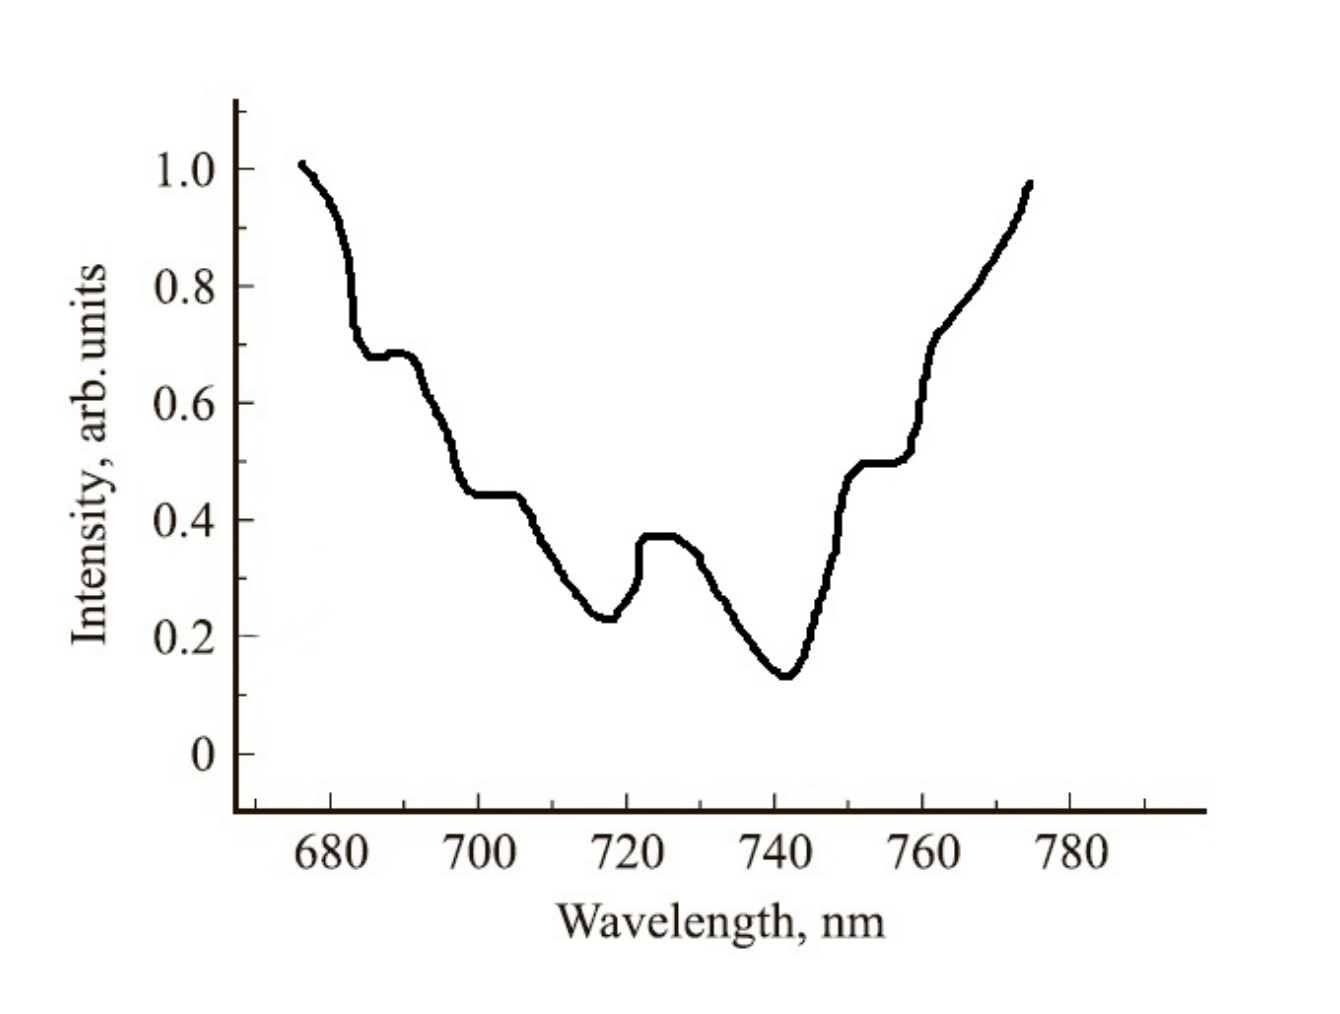
\includegraphics[width=0.8\textwidth]{graph-origin}}
  \caption{Исходный график}
  \label{graph:origin}
\end{figure}

\begin{table}[!htb]
\centering
\caption{Аргументы и значения функции}
\label{table:brightness}
\begin{tabular}{|r|r|r|r|}
  \hline
  X & Y & X & Y \\
  \hline
  679.00 & 0.98 & 731.60 & 0.30 \\
  682.37 & 0.89 & 735.78 & 0.21 \\
  683.90 & 0.76 & 741.55 & 0.15 \\
  687.85 & 0.68 & 746.10 & 0.24 \\
  692.78 & 0.65 & 748.45 & 0.33 \\
  695.88 & 0.56 & 749.92 & 0.43 \\
  700.66 & 0.45 & 754.46 & 0.49 \\
  706.78 & 0.41 & 759.47 & 0.54 \\
  711.76 & 0.31 & 761.11 & 0.64 \\
  717.53 & 0.24 & 764.30 & 0.74 \\
  721.90 & 0.30 & 768.91 & 0.82 \\
  726.31 & 0.37 & 772.98 & 0.90 \\
  \hline
\end{tabular}
\end{table}

Для построения графика (рисунок \ref{graph:brightness}) необходимо:

\begin{enumerate}
  \item В программу SciDAVis вставить полученные табличные значения.
  \item Нажать на вкладку Линия+Символы. График построен!
  \item Необходимо его оформить по правилам.
\end{enumerate}

\begin{figure}[!htb]
  \centerline{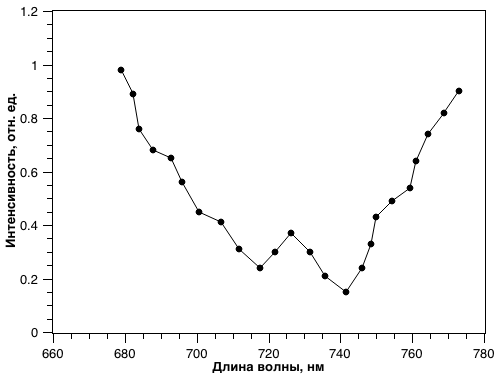
\includegraphics[width=0.8\textwidth]{graph-brightness}}
  \caption{График построенный по данным, полученным в режиме оцифровки по максимальной яркости}
  \label{graph:brightness}
\end{figure}

\subsection{Автоматический режим оцифровки по цвету}

Для того чтобы выполнить оцифровку по цвету необходимо совершить следующие действия:

\begin{enumerate}
  \item Открыть изображение в Graph2Digit.
  \item Привязать координаты по 4 точкам.
  \item На вкладке оцифровка выбрать метод — по цвету.
  \item Далее нужно выбрать область оцифровки.
  \item Выбрать любую точку на графике и кликнуть по ней два раза.
  \item Затем нажать F9, результат в таблице \ref{table:color}.
\end{enumerate}

\begin{table}[!htb]
\centering
\caption{Аргументы и значения функции}
\label{table:color}
\begin{tabular}{|r|r|r|r|}
  \hline
  X & Y & X & Y \\
  \hline
  679.14 & 0.99 & 735.33 & 0.24 \\
  682.46 & 0.92 & 742.03 & 0.16 \\
  683.70 & 0.86 & 746.69 & 0.29 \\
  689.03 & 0.69 & 749.04 & 0.42 \\
  695.63 & 0.58 & 754.81 & 0.51 \\
  702.76 & 0.45 & 760.63 & 0.65 \\
  711.64 & 0.33 & 765.27 & 0.77 \\
  718.35 & 0.25 & 771.75 & 0.89 \\
  722.18 & 0.37 & 775.36 & 0.98 \\
  727.26 & 0.37 & & \\
  \hline
\end{tabular}
\end{table}

Для построения графика (рисунок \ref{graph:color}) необходимо:

\begin{enumerate}
  \item В программу SciDAVis вставить полученные табличные значения.
  \item Нажать на вкладку Линия+Символы. График построен!
  \item Необходимо его оформить по правилам.
\end{enumerate}

\begin{figure}[!htb]
  \centerline{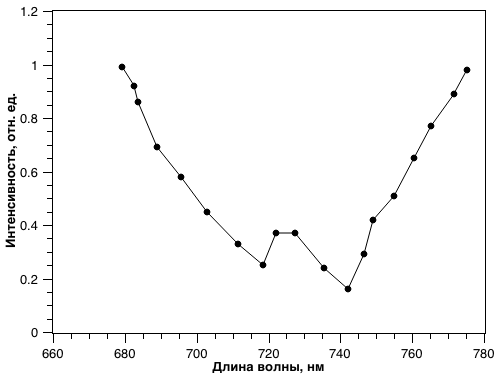
\includegraphics[width=0.8\textwidth]{graph-color}}
  \caption{График построенный по данным, полученным в режиме оцифровки по цвету}
  \label{graph:color}
\end{figure}

\subsection{Ручной режим оцифровки}

Для того чтобы выполнить оцифровку в ручном режиме необходимо совершить следующие действия:

\begin{enumerate}
  \item Открыть изображение в Graph2Digit.
  \item Привязать координаты по 4 точкам.
  \item На вкладке оцифровка выбрать метод — вручную.
  \item Далее нужно выбрать область оцифровки.
  \item И вручную пройтись по всему графику.
  \item Затем нажать F9, результат в таблице \ref{table:manual}
\end{enumerate}

\begin{table}[!htb]
  \centering
  \caption{Аргументы и значения функции}
  \label{table:manual}
  \begin{tabular}{|r|r|r|r|}
    \hline
    X & Y & X & Y \\
    \hline
    676.98 & 1.02 & 730.91 & 0.33 \\
    681.69 & 0.93 & 742.52 & 0.13 \\
    684.26 & 0.72 & 750.19 & 0.46 \\
    686.07 & 0.68 & 752.99 & 0.49 \\
    691.23 & 0.68 & 756.86 & 0.5  \\
    698.76 & 0.45 & 759.11 & 0.53 \\
    705.94 & 0.44 & 762.41 & 0.72 \\
    718.46 & 0.23 & 770.08 & 0.84 \\
    722.09 & 0.37 & 775.55 & 0.97 \\
    727.07 & 0.37 & 779.27 & 0.98 \\
    \hline
  \end{tabular}
\end{table}

Для построения графика (рисунок \ref{graph:manual}) необходимо:

\begin{enumerate}
  \item В программу SciDAVis вставить полученные табличные значения.
  \item Нажать на вкладку Линия+Символы. График построен!
  \item Необходимо его оформить по правилам.
\end{enumerate}

\begin{figure}[!htb]
  \centerline{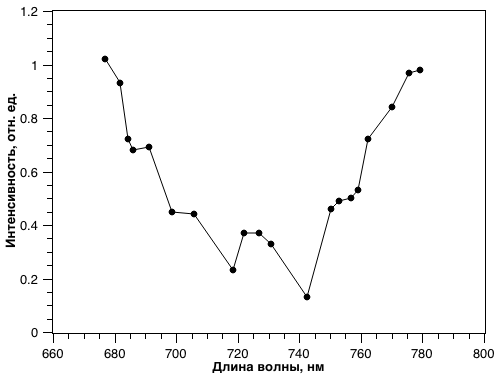
\includegraphics[width=0.8\textwidth]{graph-manual}}
  \caption{График построенный по данным, полученным в ручном режиме}
  \label{graph:manual}
\end{figure}

\section{Оцифровка произвольного графика}

\subsection{Режим оцифровки по максимальной яркости}

\begin{figure}[!htb]
  \centerline{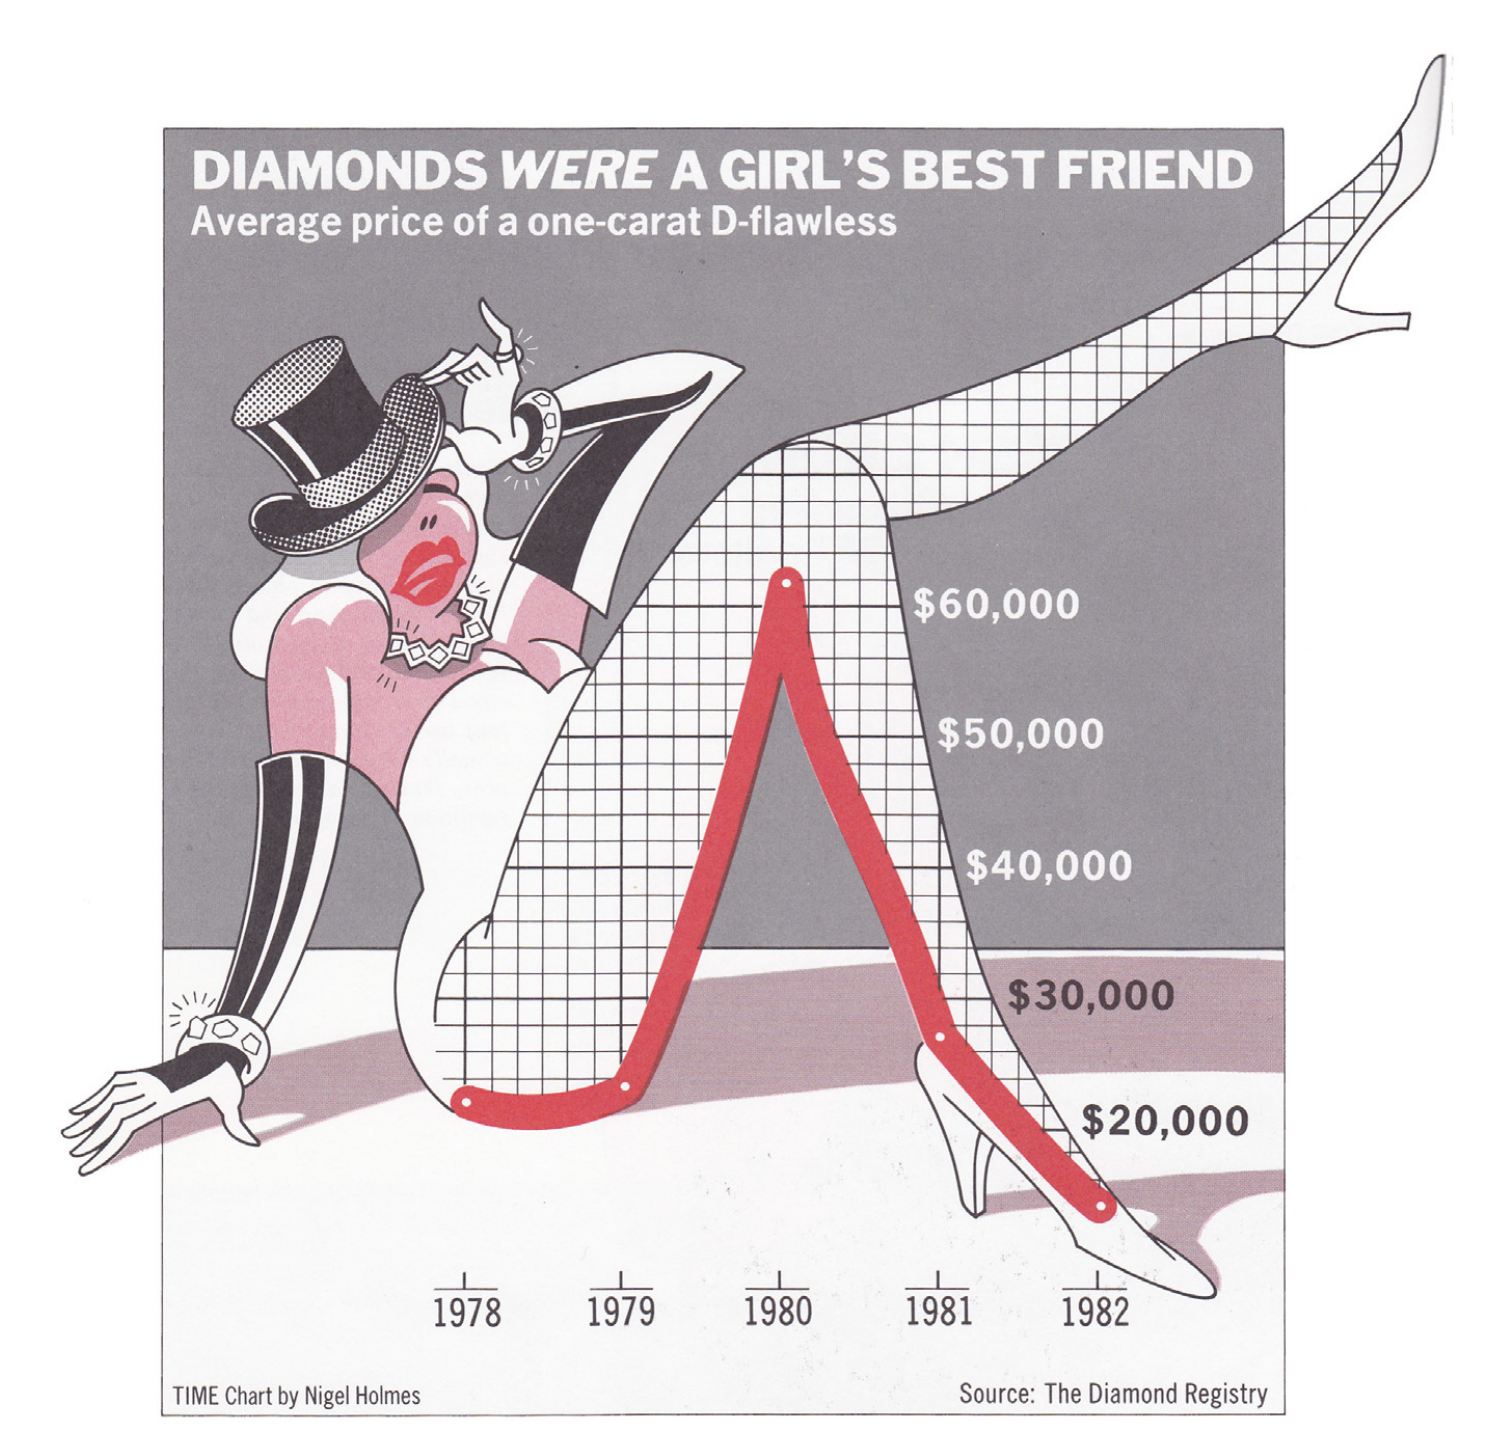
\includegraphics[width=0.8\textwidth]{graph-custom-origin}}
  \caption{Исходный график}
  \label{graph:custom-origin}
\end{figure}

Для того чтобы выполнить оцифровку по максимальной яркости необходимо совершить следующие действия:

\begin{enumerate}
  \item Открыть изображение в Graph2Digit (рисунок \ref{graph:custom-origin}).
  \item Привязать координаты по 4 точкам.
  \item На вкладке оцифровка выбрать метод — по макс. Яркости.
  \item На вкладке картинка поставить галочку на негативе.
  \item Далее нужно выбрать область оцифровки.
  \item Затем нажать F9, результат в таблице \ref{table:custom-brightness}.
\end{enumerate}

\begin{table}[!htb]
\centering
\caption{Аргументы и значения функции}
\label{table:custom-brightness}
\begin{tabular}{|r|r|r|r|}
  \hline
  X & Y & X & Y \\
  \hline
  1978.2 & 22075 & 1980.4 & 59679 \\
  1978.3 & 21172 & 1980.5 & 50178 \\
  1978.7 & 22345 & 1980.6 & 43942 \\
  1979.4 & 27973 & 1980.7 & 37775 \\
  1979.5 & 32439 & 1980.9 & 32624 \\
  1979.6 & 38738 & 1981.2 & 26656 \\
  1979.7 & 43942 & 1981.5 & 22811 \\
  1979.9 & 47636 & 1981.7 & 17275 \\
  1980.1 & 56259 & 1981.9 & 15867 \\
  1980.3 & 57487 & & \\
  \hline
\end{tabular}
\end{table}

Для построения графика (рисунок \ref{graph:custom-brightness}) необходимо:

\begin{enumerate}
  \item В программу SciDAVis вставить полученные табличные значения.
  \item Нажать на вкладку Линия+Символы. График построен!
  \item Необходимо его оформить по правилам.
\end{enumerate}

\begin{figure}[!htb]
  \centerline{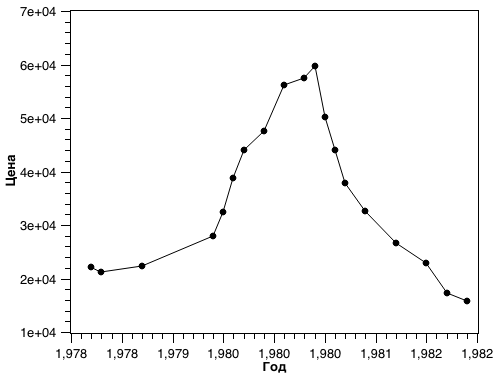
\includegraphics[width=0.8\textwidth]{graph-custom-brightness}}
  \caption{График построенный по данным, полученным в режиме оцифровки по максимальной яркости}
  \label{graph:custom-brightness}
\end{figure}

\subsection{Автоматический режим оцифровки по цвету}

Для того чтобы выполнить оцифровку по цвету необходимо совершить следующие действия:

\begin{enumerate}
  \item Открыть изображение в Graph2Digit.
  \item Привязать координаты по 4 точкам.
  \item На вкладке оцифровка выбрать метод — по цвету.
  \item Далее нужно выбрать область оцифровки.
  \item Выбрать любую точку на графике и кликнуть по ней два раза.
  \item Затем нажать F9, результат в таблице \ref{table:custom-color}.
\end{enumerate}

\begin{table}[!htb]
\centering
\caption{Аргументы и значения функции}
\label{table:custom-color}
\begin{tabular}{|r|r|r|r|}
  \hline
  X & Y & X & Y \\
  \hline
  1977.1 & 22581 & 1980.4 & 61532 \\
  1978.3 & 23741 & 1980.5 & 51755 \\
  1978.5 & 21824 & 1980.6 & 41483 \\
  1979.3 & 24212 & 1980.7 & 36872 \\
  1979.4 & 28888 & 1980.9 & 32419 \\
  1979.5 & 37596 & 1981.4 & 28136 \\
  1979.6 & 41994 & 1981.7 & 20520 \\
  1979.8 & 48200 & 1981.9 & 16381 \\
  1979.9 & 52956 & 1982.1 & 14073 \\
  1980.1 & 57145 & 1982.7 & 21662 \\
  \hline
\end{tabular}
\end{table}

Для построения графика (рисунок \ref{graph:custom-color}) необходимо:

\begin{enumerate}
  \item В программу SciDAVis вставить полученные табличные значения.
  \item Нажать на вкладку Линия+Символы. График построен!
  \item Необходимо его оформить по правилам.
\end{enumerate}

\begin{figure}[!htb]
  \centerline{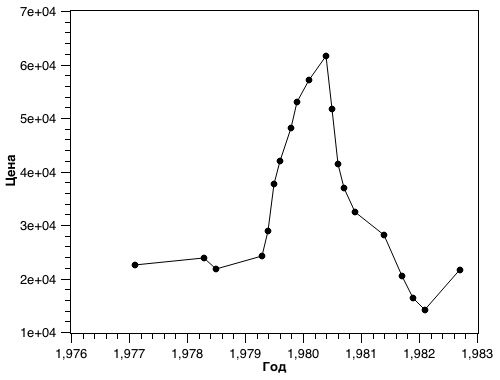
\includegraphics[width=0.8\textwidth]{graph-custom-color}}
  \caption{График построенный по данным, полученным в режиме оцифровки по цвету}
  \label{graph:custom-color}
\end{figure}

\subsection{Ручной режим оцифровки}

Для того чтобы выполнить оцифровку в ручном режиме необходимо совершить следующие действия:

\begin{enumerate}
  \item Открыть изображение в Graph2Digit.
  \item Привязать координаты по 4 точкам.
  \item На вкладке оцифровка выбрать метод — вручную.
  \item Далее нужно выбрать область оцифровки.
  \item И вручную пройтись по всему графику.
  \item Затем нажать F9, результат в таблице \ref{table:custom-manual}
\end{enumerate}

\begin{table}[!htb]
  \centering
  \caption{Аргументы и значения функции}
  \label{table:custom-manual}
  \begin{tabular}{|r|r|r|r|}
    \hline
    X & Y & X & Y \\
    \hline
    1977.0 & 22581 & 1981.1 & 27110 \\
    1978.2 & 22741 & 1981.6 & 19667 \\
    1978.5 & 23148 & 1982.8 & 14149 \\
    1978.7 & 23517 & 1980.8 & 42190 \\
    1979.3 & 23554 & & \\
    1979.6 & 42916 & & \\
    1980.2 & 61553 & & \\
    1980.6 & 54879 & & \\
    1980.7 & 44235 & & \\
    \hline
  \end{tabular}
\end{table}

Для построения графика (рисунок \ref{graph:custom-manual}) необходимо:

\begin{enumerate}
  \item В программу SciDAVis вставить полученные табличные значения.
  \item Нажать на вкладку Линия+Символы. График построен!
  \item Необходимо его оформить по правилам.
\end{enumerate}

\begin{figure}[!htb]
  \centerline{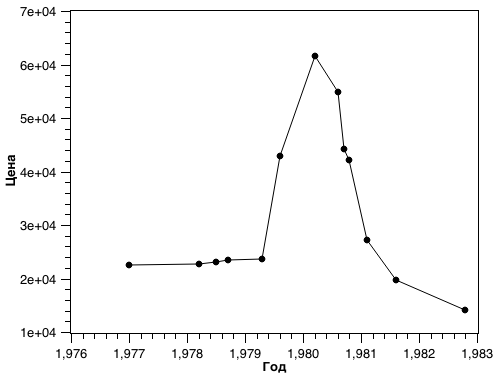
\includegraphics[width=0.8\textwidth]{graph-custom-manual}}
  \caption{График построенный по данным, полученным в ручном режиме}
  \label{graph:custom-manual}
\end{figure}

\end{document}
